\section{Fingerprint tool}
The analysis of application performance is essential to better exploit its potential on High-Performance Computing (HPC) architectures. Access to performance counters, available in modern processors, allows collecting key information about program behavior to provide the most appropriate HPC execution strategy.
In this context, we have developed an accurate tool based on performance counters, which facilitates modeling, fingerprinting, behavior comparison and clustering of applications.
It provides a high-level Python API for accessing and configuring performance counters; while execution and counters data gathering is  performed by a C++ module to reduce overhead. 
Indeed, the accuracy of this multiplatform tool was also compared to existing alternatives.  
Key features, such as performance counters collection, post-processing, and comparison, enable fingerprinting of applications, an important step in understanding program behavior for later classification and optimization according to the parameters characterizing the target HPC platform.
For demonstration purposes, the tool was used in the clustering of Polybench applications, a frequently used benchmark set for kernels monitoring. 
%%, a frequently used benchmark for compiler optimization and testing. 
This clustering facilitated the identification of applications with similar and comparable behaviors in terms of input size, data access and transfer, resource utilization and computation, which facilitates the creation of test sets for a given environment based on specific measurement parameters.


%%%%%%%%%%%%%%%%%%%%%%%%%%%%%%%%%%%%%%%%%%%%%%%%%%%%%%%%%%%%%%%%%%%%%%%%%%%%%%%%
\subsection{Introduction}

Hardware Performance Counters are special registers available on most modern processors capable of counting micro-architectural events such as instructions executed, cache-hit, branches miss-predicted, energy estimation and much more.  In new architectures, there are hundreds of hardware events that can be monitored, and more are added to each new generation. 
Performance counters were initially introduced for debugging, but since then they have provided a lot of useful information about running applications without slowing down the execution.
They have been used in several other areas, such as software profiling \cite{Melo2010Perf, Kufrin2005Perfsuite, Knupfer2011Scorep}, CPU power modeling \cite{Zamani2012ASystems}, dynamic frequency and voltage scaling, vulnerability research and malware defense \cite{Demme2013OnCounters}.

%\cite{Geimer2010, Geimer2010TheArchitecture, Shende2006TheSystem}

Exploiting Performance Monitoring Units (PMU) requires an intimate knowledge of the micro-architecture and kernel API, as well as an awareness of an ever increasing complexity. 
Otherwise, the measurement performance and accuracy will be seriously affected. Although many tools have been developed using performance counters, programmable interfaces capable of providing good accuracy are still lacking, especially for high-level programming languages. Indeed, apart from PAPI \cite{Weaver2013Non-determinismImplementations, Mucci1999PAPI} and Perfmon \cite{Eranian2008Perfmon2} there are only a few APIs allowing access to these counters, and many others are poorly documented, unstable, or designer for a specific purpose.

Performance metrics may have different definitions and programming interfaces on different platforms. 
Therefore, besides gathering information, post-processing modules are also needed. 
Such modules will overcome the lack of precision of counters on some architectures, as indicated in \cite{Weaver2008CanTrusted,Weaver2013Non-determinismImplementations,Das2019SoK:Security}. 
Events that must be precise and deterministic (such as retired instructions) show a variation on run-to-run and over-count on x86\_64 machines, even in strictly controlled environments. These effects are almost always non-intuitive to casual users and pose problems when strict determinism is desirable. 

To meet the above mentioned requirements, our strategy combines low-level, efficient and accurate access to PMUs, facilitated by high-level programmable interfaces. This allows the user to perform all configurations and post-processing in Python,  while the underlined architecture details and information gathering are supported by a C++ module, thus preserving accuracy with limited overhead. 
In order to understand the behavior of programs for future comparisons and classification, the proposed tool makes another contribution: the ability to fingerprint and cluster applications.

The definition of reference parameters, such as input size of programs, and performance measures uniformization, allow us to cluster benchmarks such as PolyBench \cite{Gonzalez2021PolyBench}, a collection of numerical computations with static control flow extracted from various application domains, with interesting results. 
In addition to contributing to the standardization of kernel execution and monitoring, this clustering has identified applications with similar and comparable behavior in terms of input size, data transfer and access, resources used and computation; which facilitates the creation of test sets for a given environment, according to specific measurement parameters. 

The rest of this article is organized as follows. subsection 2 provides the related work regarding tools available and requirements. subsection 3 presents the performance counters and motivation. subsection 4 presents our clustering and application analysis tool, architecture and components. subsection 5 shows evaluation results: the comparison of existing API and the clustering of the PolyBench benchmarks. Finally, subsection 8 concludes this article.

\subsection{Related Work}

There are only a few APIs allowing access to performance counters.
PAPI \cite{Weaver2013Non-determinismImplementations, Mucci1999PAPI}, one of the most used libraries for accessing hardware performance counters, was originally developed to provide portable access to the counters found on a diverse collection of modern microprocessors. Rather than learning and writing a new performance infrastructure every time it is ported to a new machine. Measurement code can be written in the PAPI API, which hides the underlying interface.  
PAPI was developed on C and a few non-official libraries were ported to Python. The main problem we found using PAPI was the Python version of has a considerable overhead, it also does not have an easy way to create raw events or low-level control without having to use a special driver. And as our tests will show later, counters sampling over time does not produce good results either.

There are also available a set of interfaces using their own drivers, mainly because the counters are only accessible in kernel mode (ring 0) to control the events for which the counter must be started or stopped. Some events are fixed and others require the development of a dedicated kernel driver. 

Perfctr \cite{Nikolaev2011Perfctr} supports per-kernel-thread and system-wide monitoring for most major processor architectures. It is distributed as a stand-alone kernel patch. The interface is mostly used by tools built on top of the PAPI performance toolkit. 

The Intel VTUNE \cite{Intel2021Vtune} performance analyzer comes with its own kernel interface, implemented by an open-source driver. The interface supports system-wide monitoring only and is very specific to the needs of the tool.

The problem with the approach of a tool and its own kernel interface is dangerous because, as mentioned on \cite{Eranian2008Perfmon2}, there is clearly code duplication, but more importantly, there is no coordination between the various interfaces that may coexist sharing access to the same PMU resource. To solve this problem, Perfmon2 \cite{Eranian2008Perfmon2} offers a standard interface that all tools can use. Unfortunately, it has not been widely adopted, just supported by a few architectures like the IA64. Instead, Linux comes up with a performance counters subsystem which provides a complete set of configurations.


\subsection{Reading Performance Counters}

Although hundreds of events are available for monitoring, only a limited number of counters can be used simultaneously.
Therefore, the events to be monitored should be carefully selected and configured using the available counters.

The number of counters available varies between processor architectures, e.g., modern Intel CPUs \cite{Intel2013IntelGuide} support three fixed and four programmable counters per core. Fixed counters monitor events such as Instruction Retired (how many instructions were completely executed), logical cycles, and reference cycles, while programmable counters can be configured to monitor architectural and non-architectural events. 
However, if additional counters are needed, the available ones must be multiplexed.
The configuration of the counters is done by writing in Model-Specific Registers (MSR), only accessible in ring 0 (kernel mode) as indicated previously. 


% \begin{itemize}
%     \item rdmsr - Reads the contents of a 64-bit model specific register (MSR) specified in the ECX register into registers EDX:EAX. This instruction must be executed at privilege level 0 or in real-address mode
%     \item rdpmc - Is slightly faster that the equivalent rdmsr instruction. rdpmc can also be configured to allow access to the counters from userspace, without being privileged.
% \end{itemize}

Operating systems provide an abstraction of these hardware capabilities to access counters and MSRs. 
On the Linux system, where our work was developed, there is a performance monitoring subsystem which provides per-task and per CPU counters, counter groups, and related event features. 
All events are seen as 64-bit virtual counters, regardless of the width of the underlying hardware counters. 
They are accessible via special file descriptors, one file descriptor per virtual counter, opened via the perf\_event\_open() system call.  %These system call do not use rdpmc, but rdpmc is not necessarily faster than other methods of reading event values.
Counter events can be processed by interrupt, polling or on time. The interrupt operates by hooking a user-defined function to a specified event, such as a counter overflow, and whenever this event happens, a signal will be generated passing the control to the designated handler function. With polling, whenever an event occurs on the system, the counter value is queued by the operating system and the user can read from this queue using a system call. The last option is to sample over time reading counters every n second.

Ideal hardware performance counters provide exact deterministic results. Real-world PMU implementations do not always live up to this ideal \cite{Weaver2008CanTrusted, Weaver2013Non-determinismImplementations, Das2019SoK:Security, McGuire2009AnalysisKernel}. Events that should be exact and deterministic (such as the number of executed instructions) show run-to-run variations and over counts on x86 64 machines, even when running in strictly controlled environments. 
These effects are non-intuitive to casual users and cause difficulties when strict determinism is desirable, such as when implementing deterministic replay or deterministic threading libraries. 
Because of that, we have implemented a methodology to reduce the noise and over counts on performance counters.


\subsection{Implementation}

%This module provide a high-level abstraction API to Linux perf events without overhead while executing

This tool is composed of 5 modules the are Profiler, Events, Workload, Analyzer and libpfm4. 
The Workload and libpfm4 module are developed on C/C++ and interfaced with python using Python C API with SWIG (a software development tool to connects programs written in C/C++ with a variety of high-level programming languages). 
The libpfm4 module, developed by \cite{Eranian2008Perfmon2}, is used as an auxiliary library.

%The main features that this library provide is a precise synchronous start the application and counter the event, a low overhead on sampling the events on time and an easy way to find and configure event in groups or standalone. 

\subsubsection{ARCHITECTURE}

In figure \ref{fig:achitecture} we can see how these modules interact with each other.
\begin{figure}[H]
    \centering
    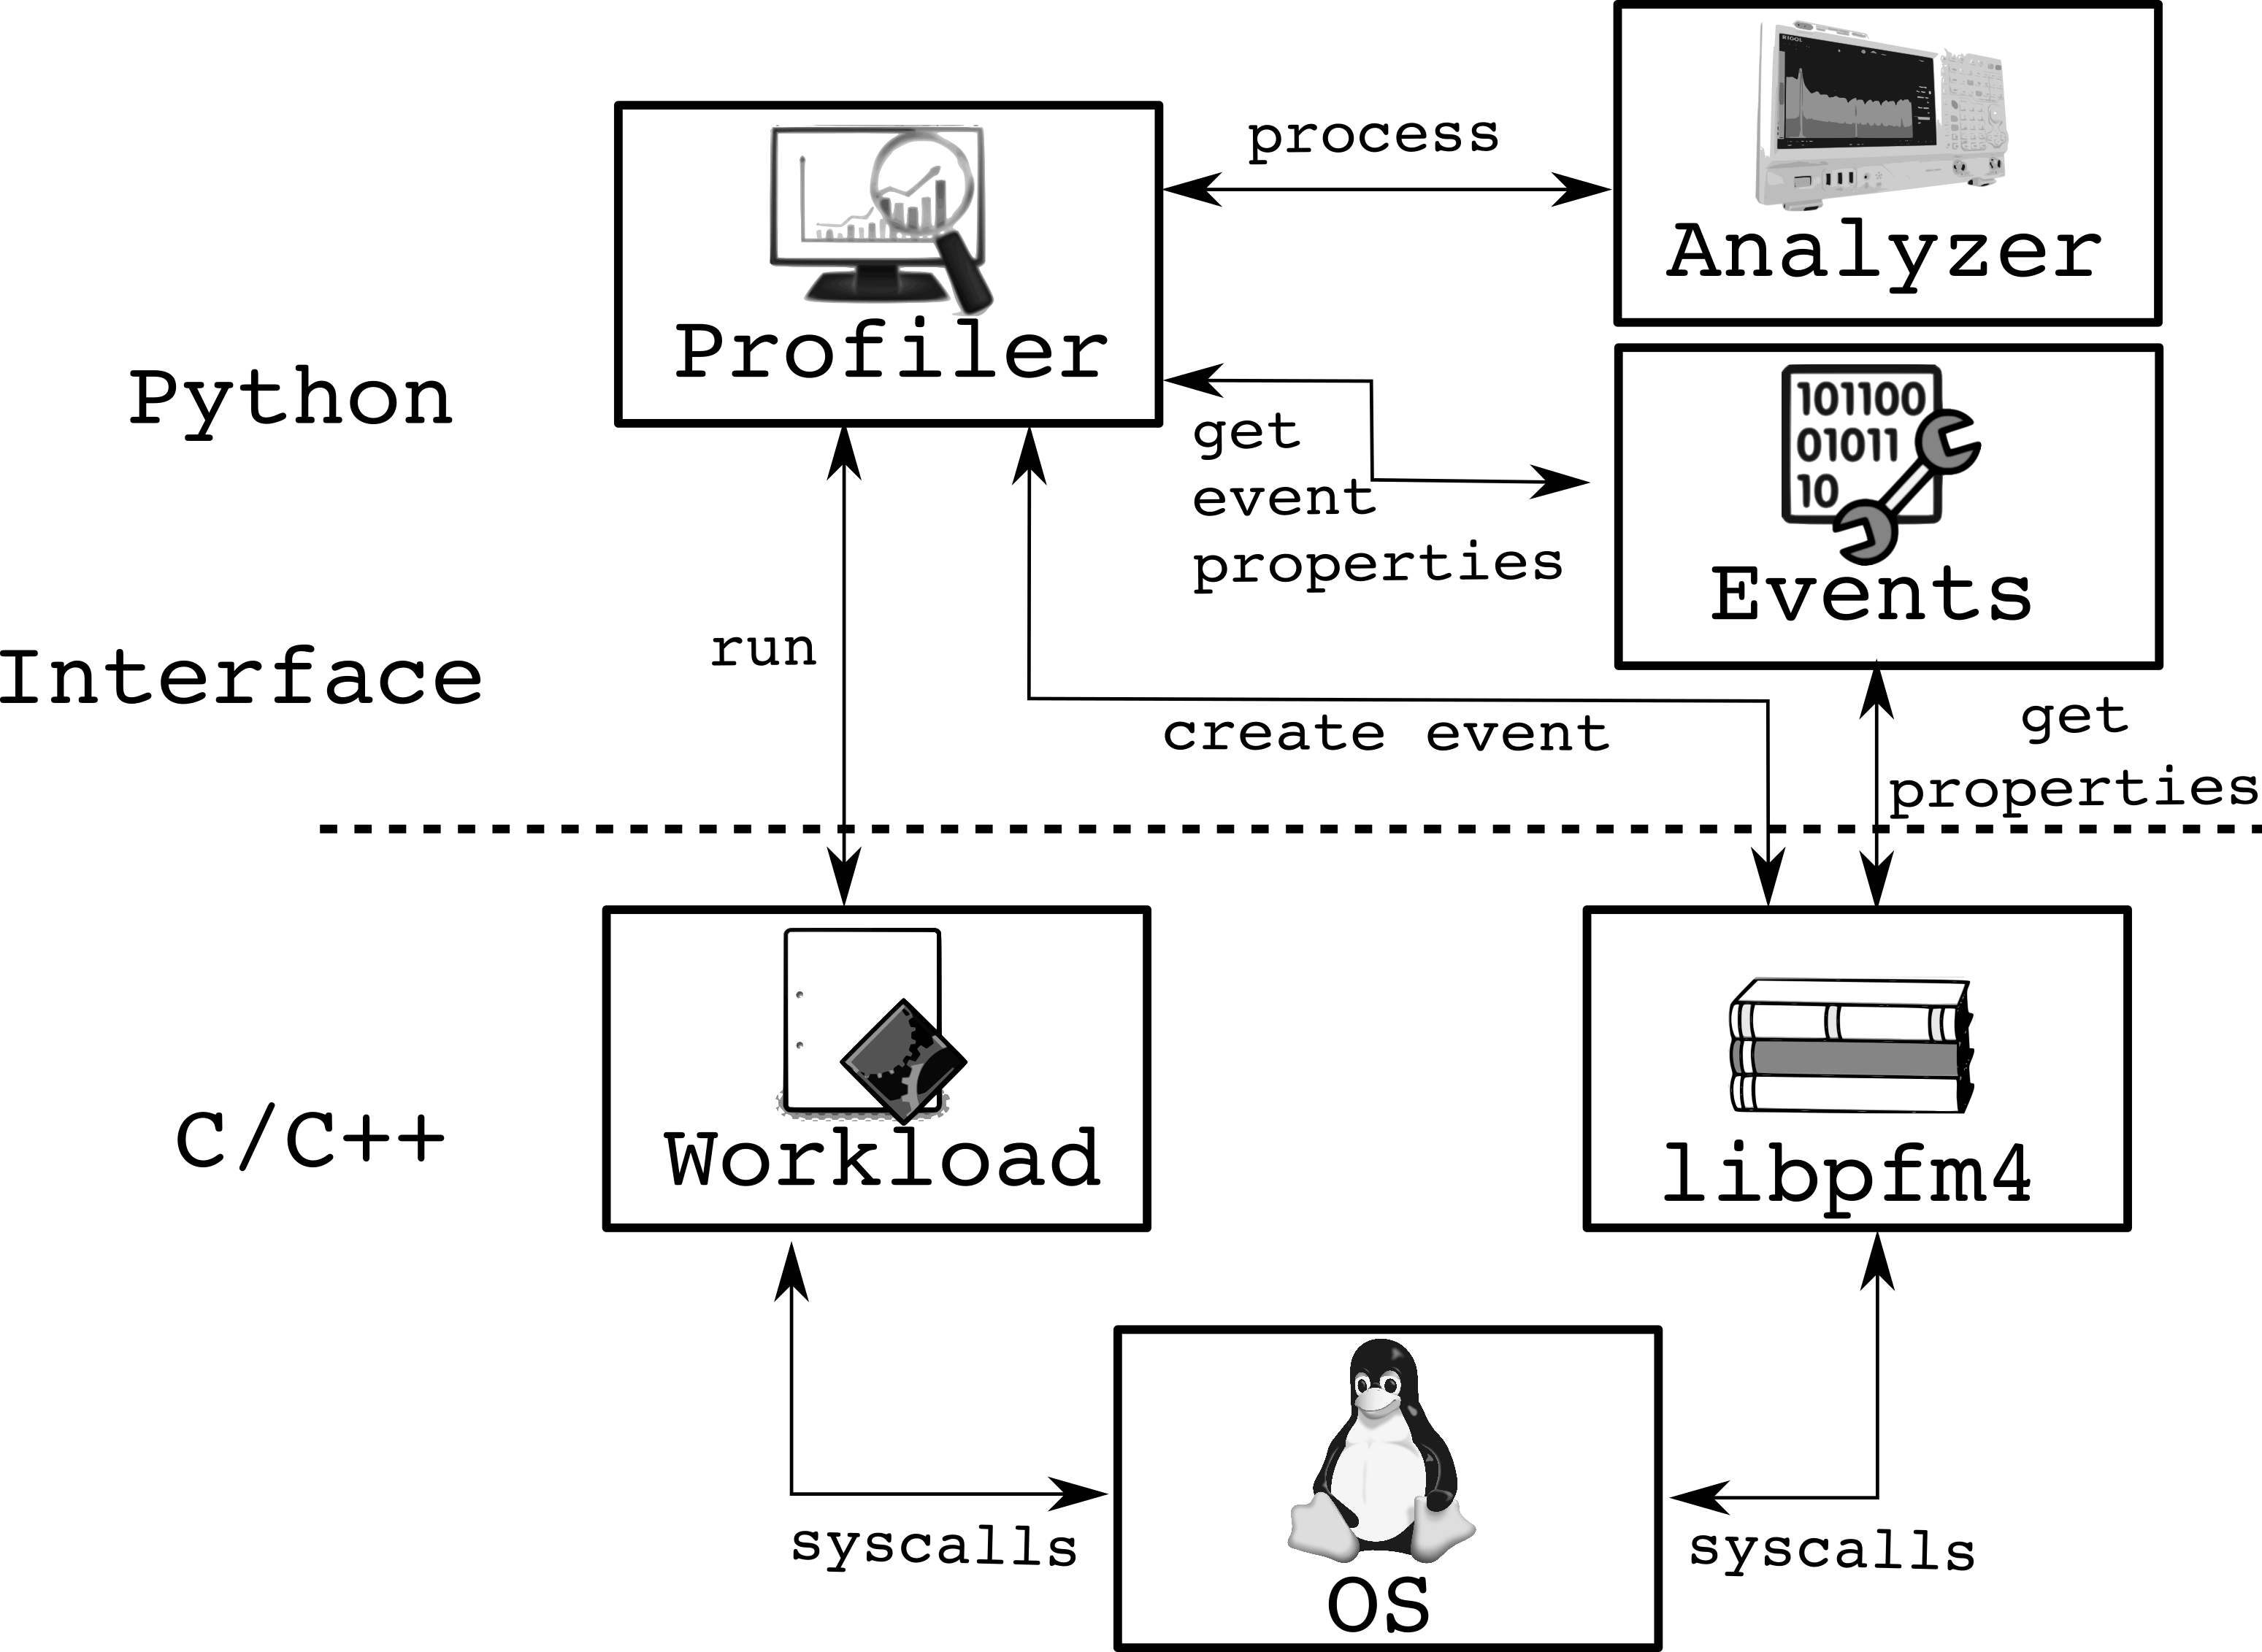
\includegraphics[width=\textwidth]{fingerprint/figures/architecture.png}
    \caption{Modules interconnection}
    \label{fig:achitecture}
\end{figure}

The Profiler is the user interface for configuring and creating events.
It is also responsible for calling the Workload module to run the application and retrieve the data after the execution is complete.

The Workload module, developed on C++, is the core of the library.
It is responsible for creating the application and the sampling process.
It provides a precisely synchronized start, it halts the program before the execution of the first instruction, using the debug interface on Linux (place), and launches the application once the counters have been properly reset and ready to run.
This module, built-in as a Python module using the Python C API, defines a set of functions, macros, and variables to access most aspects of the Python run-time system.
% The workload run simplified code
% \begin{lstlisting}[language=c++]
% reset_counters();
% start_counters();
% start_application();
% while(application.is_running()){
%      sleep(secounds);
%      sample_counters();
% }
% return sampled data;
% \end{lstlisting}
The Event module provides a description of events, events parameters, configurations and PMUs available.

System calls for reading and event creation are done directly by the Workload module or through the libpfm4 Python link. 
The libpfm4 is also used to find events encodings and convert an event name (expressed as a string) to the corresponding event encoding, either as a raw event number (as documented by the hardware vendor) or the OS-specific encoding.
In the latter case, the library is able to prepare the OS-specific data structures needed by the kernel to setup the event.

The Analyzer module is responsible for the post-processing of the data. 
It takes the data from several runs of the application and provides a set of functions to remove outlines, interpolate, filter and compare.
% \subsubsection{FUNCTIONALITY}
% This subsection is going to describe the main functionality of the API.
% Profiler module:
% \begin{lstlisting}[language=Python]
% Profiler(events_groups, program_args=None)
% \end{lstlisting}
% This constructor creates a profiler object from a list of events groups with their names, optionally can pass the application that will be executed.
% \\
% \begin{lstlisting}[language=Python]
% set_program(program_args)
% \end{lstlisting}
% Set the program and his arguments to be executed from a list.
% \\
% \begin{lstlisting}[language=Python]
% start_counters(pid=0)
% \end{lstlisting}
% Monitor events by pid. If pid its set to 0, monitor the entire system.
% \\
% \begin{lstlisting}[language=Python]
% enable_events()
% disable_events()
% reset_events()
% read_events()
% \end{lstlisting}
% Control events
% \\
% \begin{lstlisting}[language=Python]
% run(sample_period, reset_on_sample=False)
% \end{lstlisting}
% Run the application and sample the events on the time, it receives the sample time and if a flat that controls the reset on the sample. It returns the data with the events sampled. 
% \\
% \begin{lstlisting}[language=Python]
% run_background()
% \end{lstlisting}
% Run the application in background
% \begin{lstlisting}[language=Python]
% run_program(...)
% save_data(data, name)
% \end{lstlisting}
% Simple functions to run a program multiple times and store the results in a file.
% \\
% \\
% Events module:
% \begin{lstlisting}[language=Python]
% get_supported_pmus()
% get_supported_events(name)
% get_event_description(name)
% get_event_attrs(name)
% \end{lstlisting}
% These functions return a list with a description for the PMU, event, and attributes.
% \\
% \\
% Analyser module:
% \begin{lstlisting}[language=Python]
% load_data(name)
% \end{lstlisting}
% Load the data capture into an Analyser object.
% \\
% \begin{lstlisting}[language=Python]
% process(verbose=False)
% \end{lstlisting}
% Process the data, using the method described on the post-processing subsection \ref{sec:posprocessing}.
% \\
% \begin{lstlisting}[language=Python]
% compare(a1, a2, feature, npoints)
% \end{lstlisting}
% Compare two objects on a specific feature.

\subsubsection{POST-PROCESSING}
\label{sec:posprocessing}
% With this API we create clusterize the applications of Polybench applications.

With the data collected from multiple runs of the application, the first goal is to obtain a single curve that minimizes the noise caused by the operating system and inaccuracies of the counters. 
In figure \ref{fig:multiple_exec} we can see the raw result of multiple runs of the Polybench 2mm program measuring the number of executed instructions. 
For better visualization, the horizontal axis has been normalized over the interval from 0 to 100. 
This implies that we no longer analyze the program on the time scale, but in the interval in which it took place.

\begin{figure}[H]
    \centering
    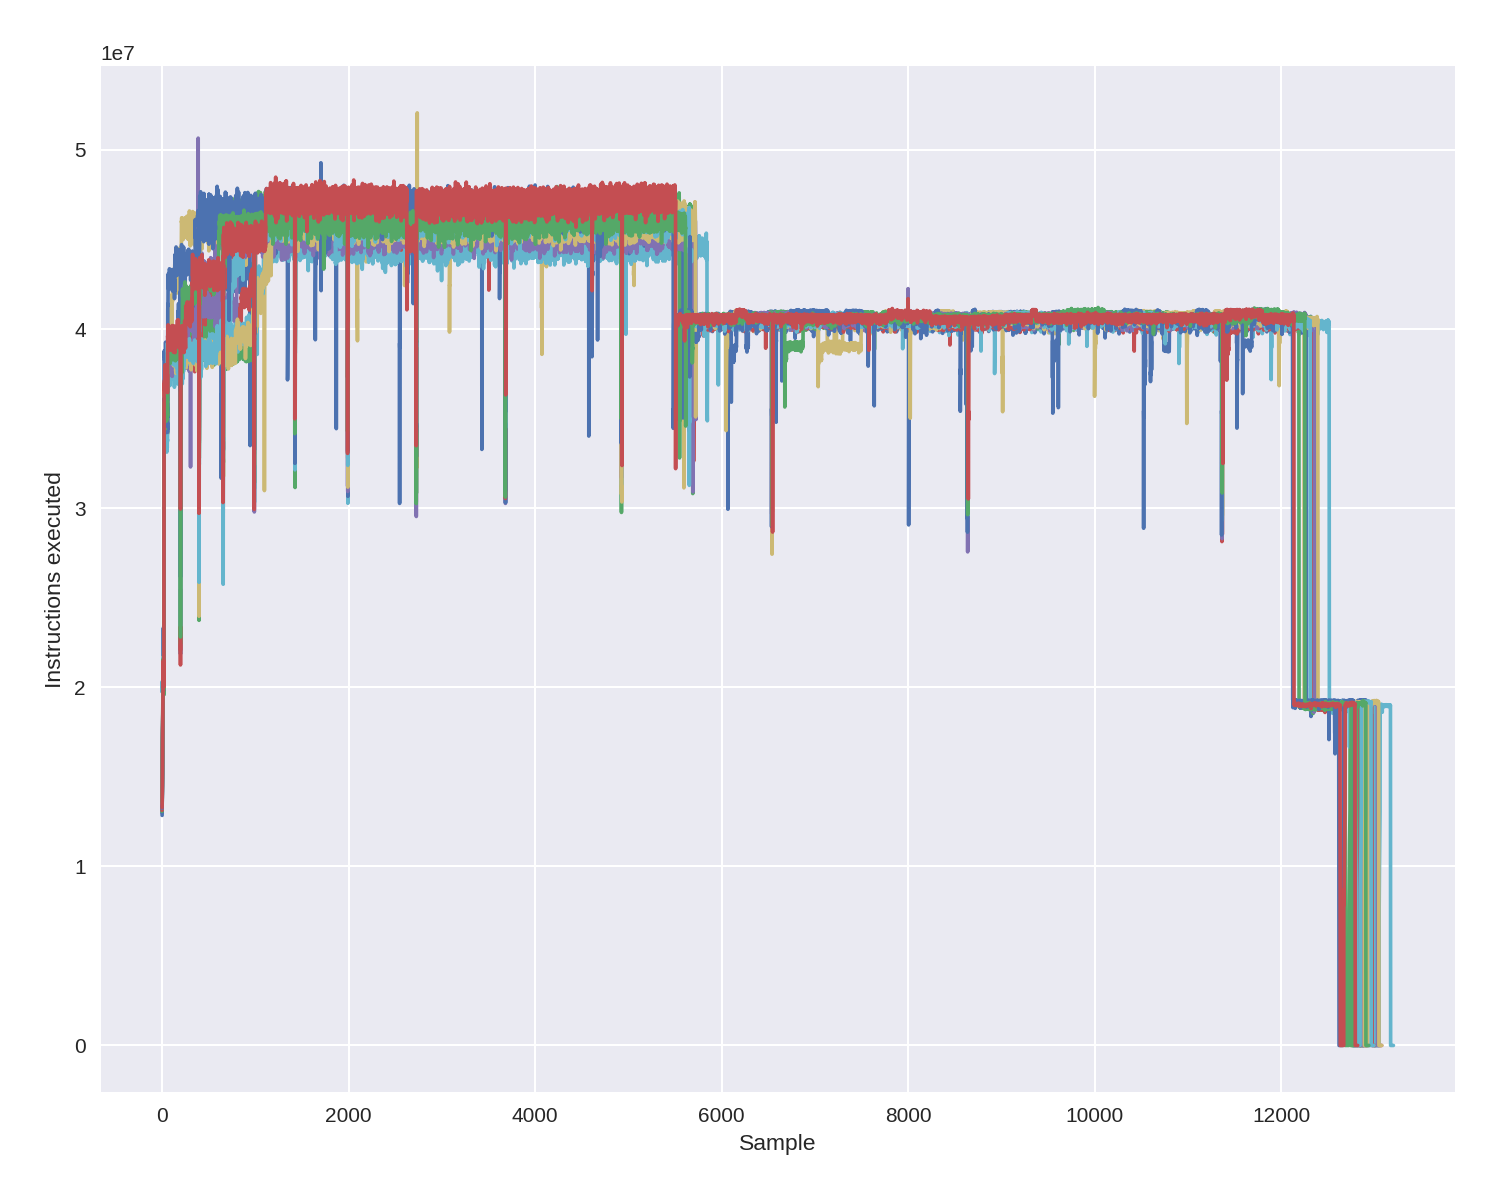
\includegraphics[width=\textwidth]{fingerprint/figures/workflow.png}
    \caption{Multiple executions of the Polybench 2mm program with different input sizes}
    \label{fig:multiple_exec}
\end{figure}

We apply a median filter to each set of runs, sorting the values and removing edge values.
Then we calculate the average curve, whose final result can be observed on the figure \ref{fig:single_curve}.

\begin{figure}[H]
    \centering
    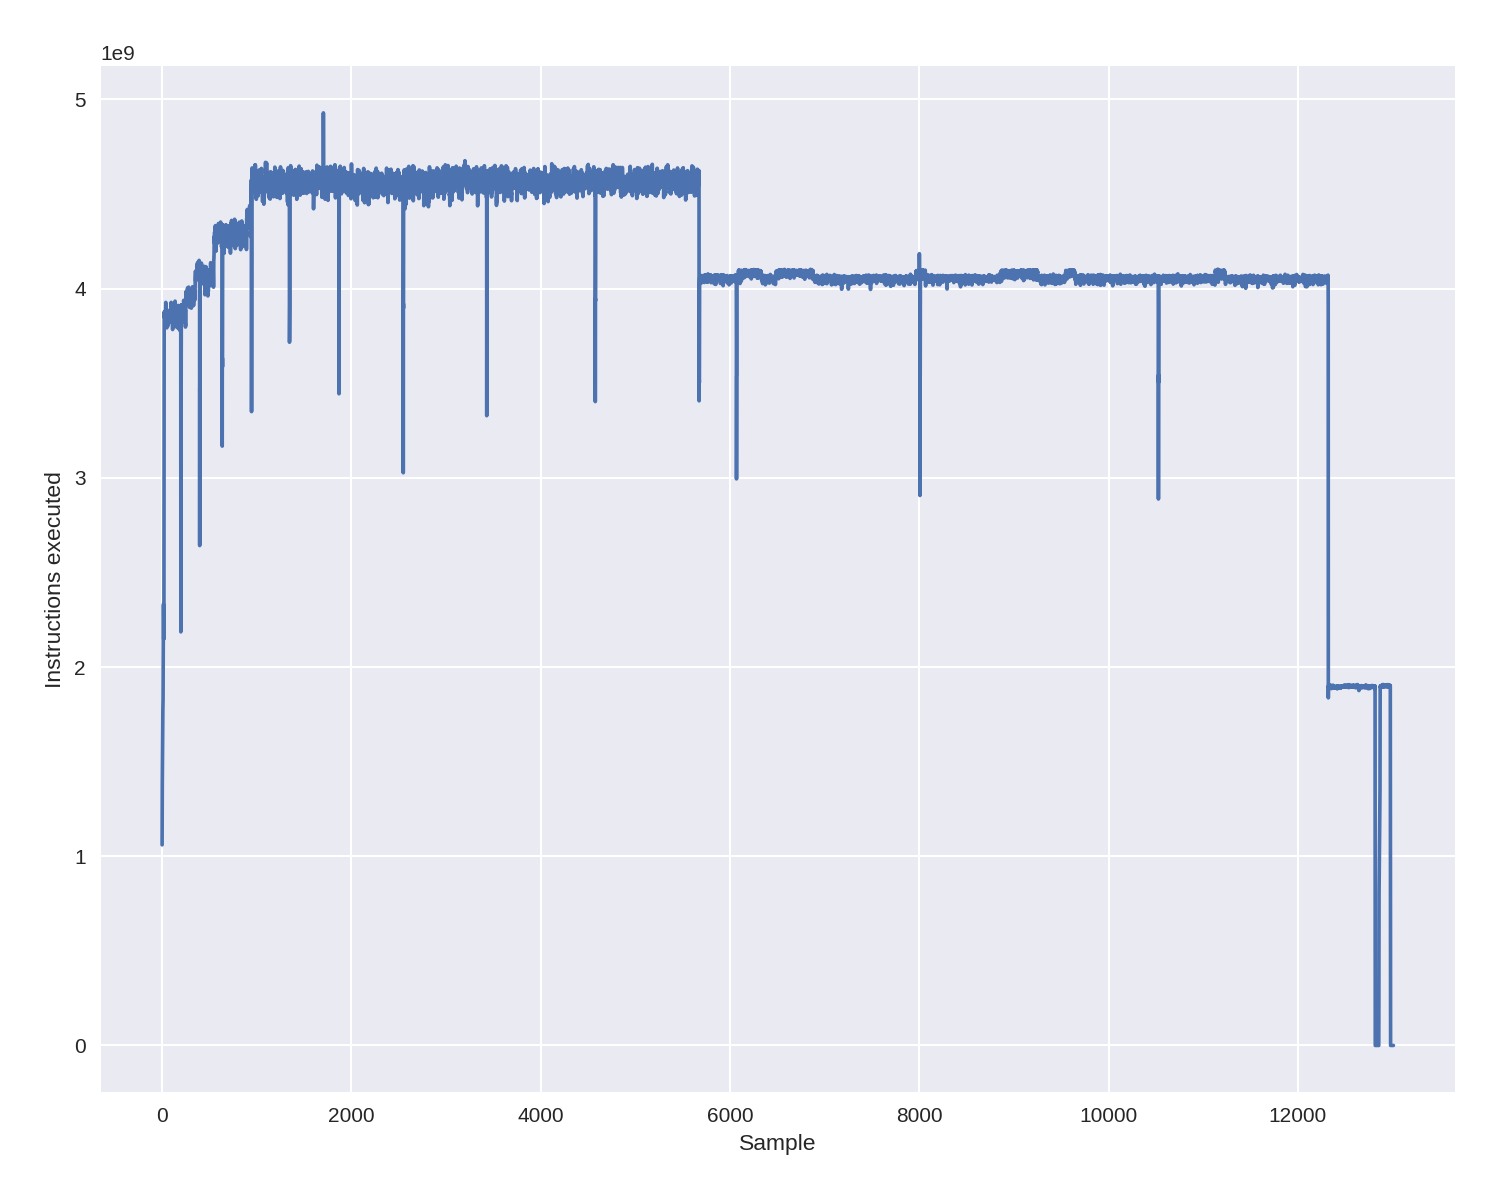
\includegraphics[width=\textwidth]{fingerprint/figures/workflow_1.png}
    \caption{Single instance representation}
    \label{fig:single_curve}
\end{figure}

 After that, we interpolate the curve using the B-spline \cite{Hang2017CubicApplications} algorithm to get the same number of points to all curves. 
 The result of this step can be observed in figure \ref{fig:interporlation}. 

\begin{figure}[H]
    \centering
    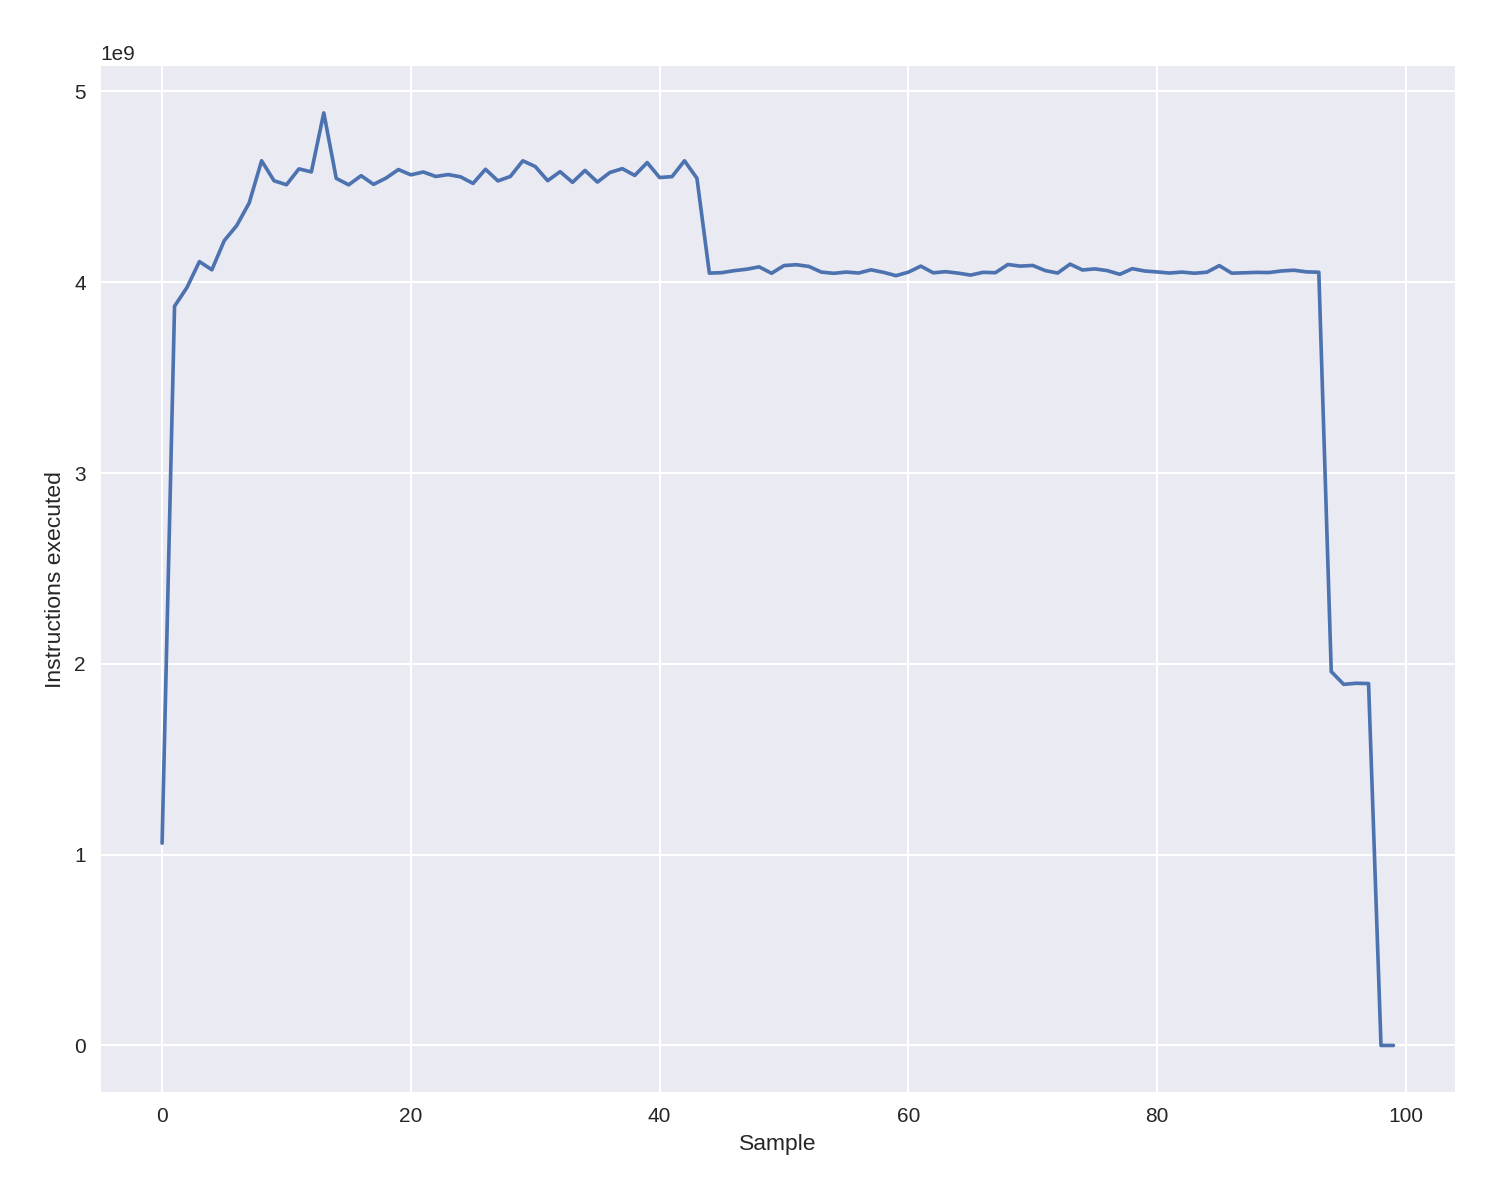
\includegraphics[width=\textwidth]{fingerprint/figures/workflow_2.png}
    \caption{Interpolation}
    \label{fig:interporlation}
\end{figure}

Finally, we use the Savgol filter \cite{Luo2005PropertiesDifferentiators} in order to smooth the data to increase the signal-to-noise ratio without too much distortion. The result is shown in figure \ref{fig:filtering}.

\begin{figure}[H]
    \centering
    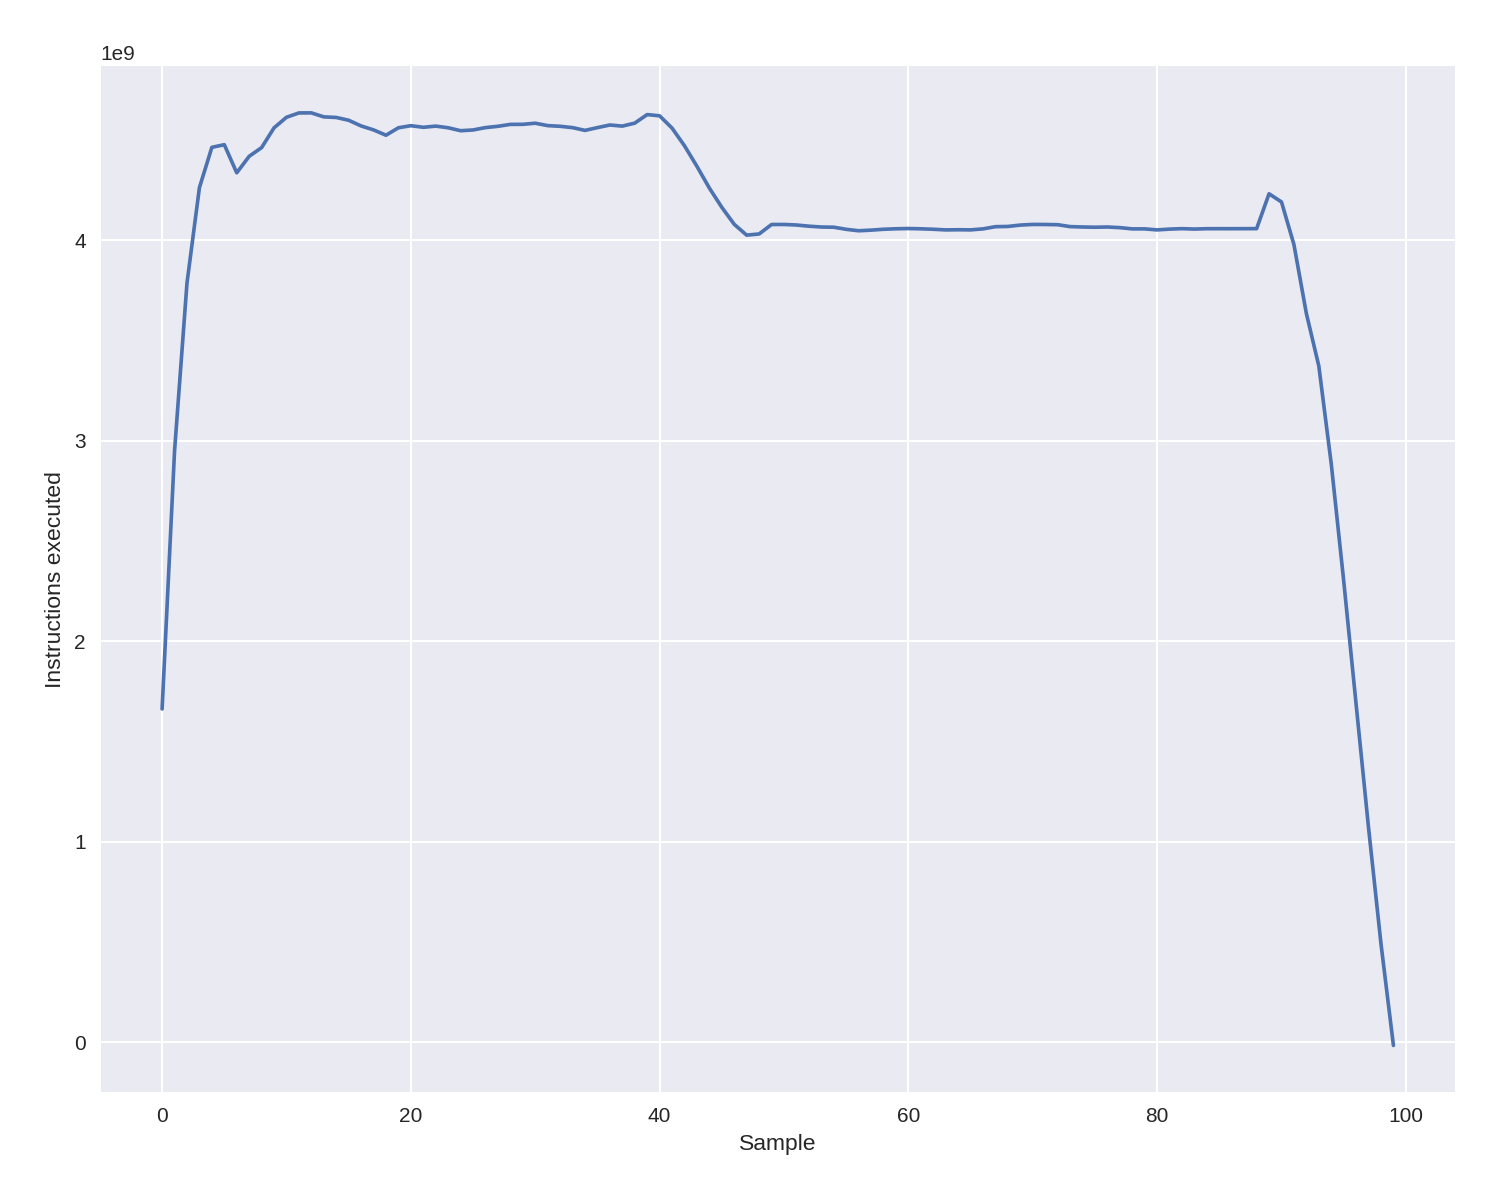
\includegraphics[width=\textwidth]{fingerprint/figures/workflow_3.png}
    \caption{Filtering}
    \label{fig:filtering}
\end{figure}




